%\section{Bathtub model}
%In the previous section we studied the possibility of using a polynomial to capture the relationship between grain size, number of cores, and throughput for a fixed matrix size, with the purpose of finding a range of grain size that leads us to maximum performance. 
%Although the polynomial function was helpful in directing us toward our objective, it does not have a physical implication. 
%
%This motivated us to change our view, and instead of looking just at the data and trying to find a function to fit the data, study the behavior of the data, and then find a function that would be likely to fit the data. That function would be a good fit mostly because that's how we expect the throughput to change with grain size, and not just how the data looks like.   
%
%As stated in Section~\ref{task}, Grubel et.al.\cite{grubel2015performance} has studied the task granularity for a specific problem(1D stencil). Looking at the graph representing the execution time based on the grain size, which resembles a bathtub, we are interested in formulating this graph based on our understanding of the effect of task granularity. Figure~\ref{fig21} shows the execution time in terms of grain size for $DMATDMATADD$ benchmark for matrix size $690\times690$ on $4$ cores.
%
%\vspace{\baselineskip}	
%\begin{figure}[H]
%	\centering
%	\subfloat[]{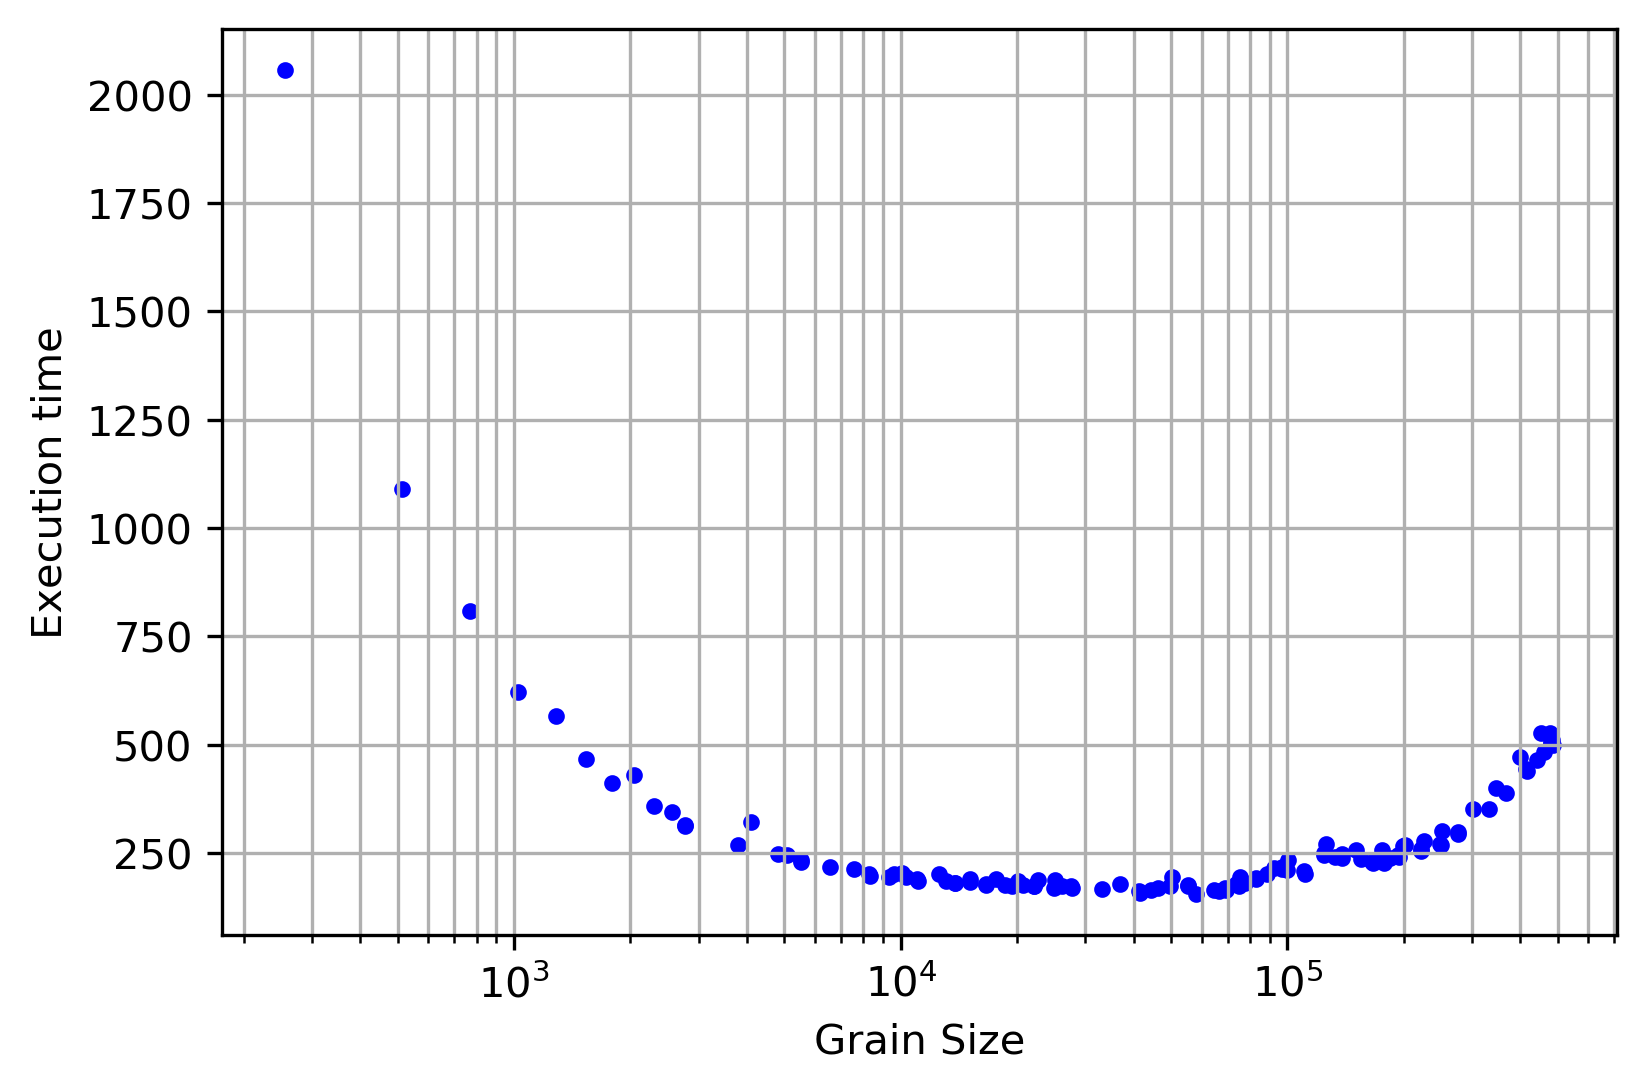
\includegraphics[scale=.5]{images/bathtub/all_690_4.png}\label{fig20:a}}
%	\subfloat[]{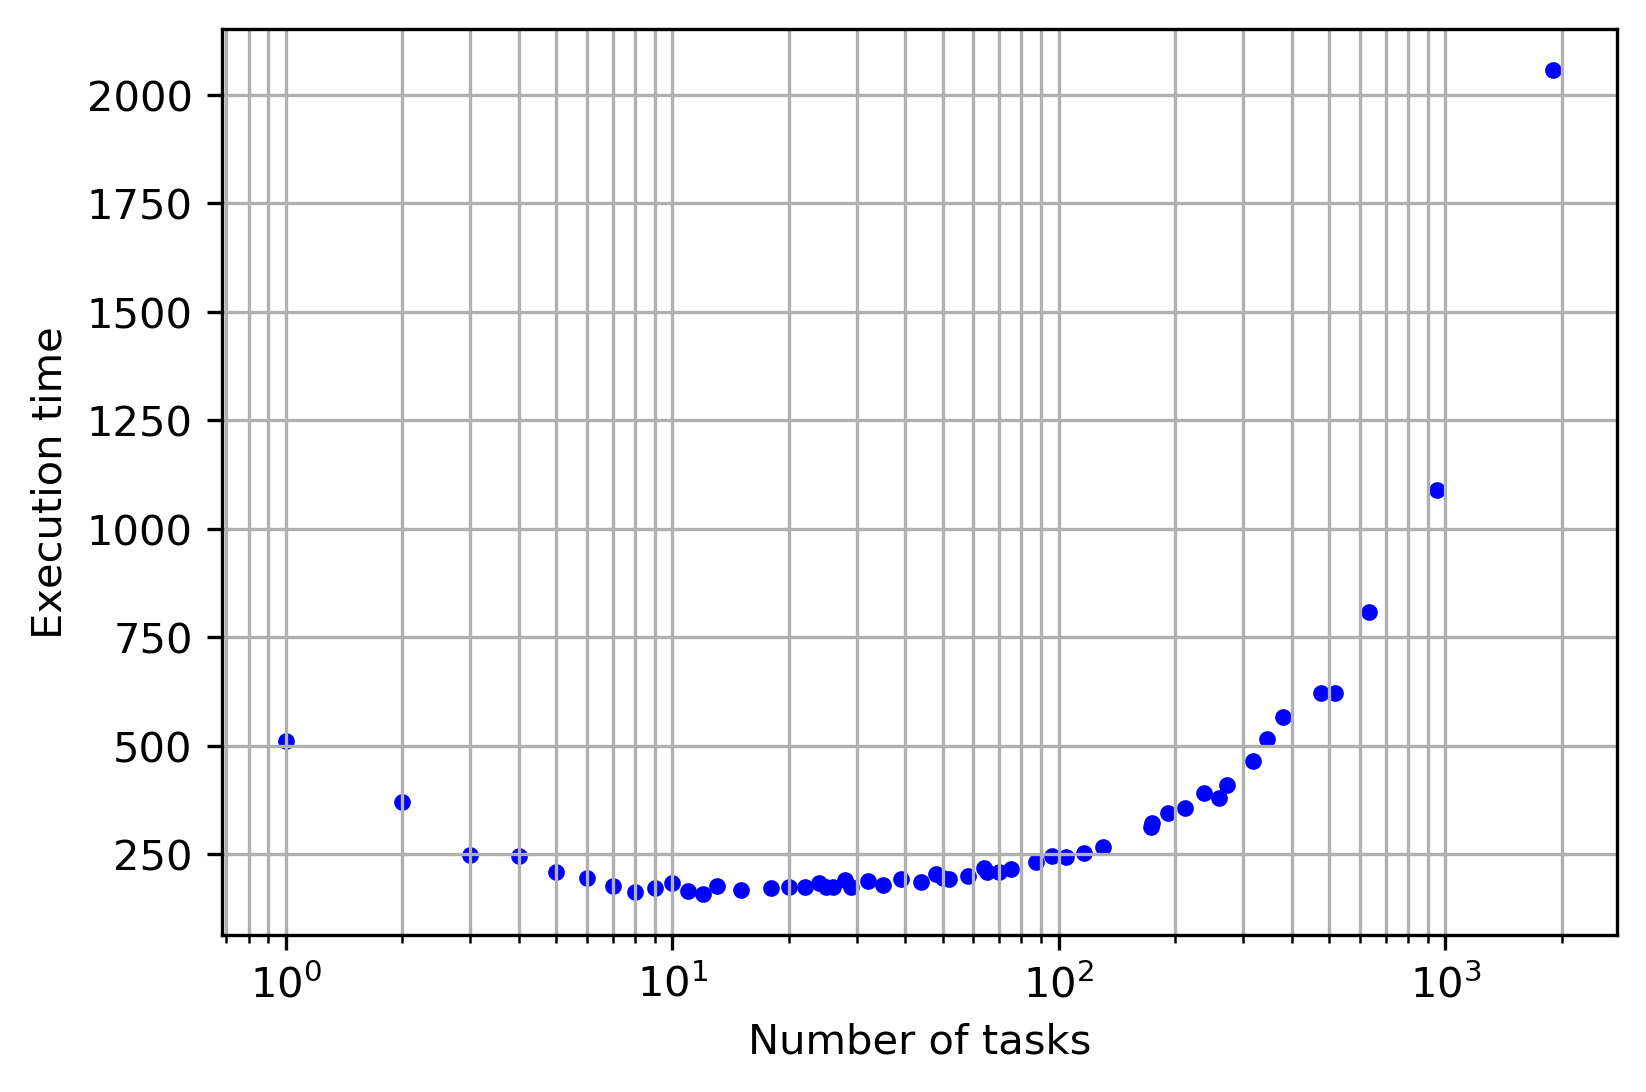
\includegraphics[scale=.5]{images/bathtub/tasks_all_690_4.png}\label{fig20:b}}
%	\caption{(a)The execution time vs. grain size graph, and (b) execution time vs. number fo tasks graph for $DMATDMATADD$ benchmark for matrix size $690\times690$ ran on $4$ cores.}	
%	\label{fig21}
%\end{figure}
%
%\vspace{\baselineskip}	
%For the sake of simplicity, we change the x axis from grain size to number of tasks. Each specific grain size would create a specific number of tasks(HPX threads), since the parameters we are interested in are directly associated with he number of tasks, we represent execution time based on number of tasks, as shown in Figure~\ref{fig20:b}.
% 

